\documentclass[10pt,twocolumn,letterpaper]{article}

\usepackage{cvpr}
\usepackage{times}
\usepackage{epsfig}
\usepackage{graphicx}
\usepackage{amsmath}
\usepackage{amssymb}
\usepackage{mathtools}
\usepackage{array}
\usepackage{multirow}
\usepackage{float}


% Include other packages here, before hyperref.

% If you comment hyperref and then uncomment it, you should delete
% egpaper.aux before re-running latex.  (Or just hit 'q' on the first latex
% run, let it finish, and you should be clear).
\usepackage[breaklinks=true,bookmarks=false]{hyperref}

\cvprfinalcopy % *** Uncomment this line for the final submission

\def\cvprPaperID{****} % *** Enter the CVPR Paper ID here
\def\httilde{\mbox{\tt\raisebox{-.5ex}{\symbol{126}}}}


% Pages are numbered in submission mode, and unnumbered in camera-ready
%\ifcvprfinal\pagestyle{empty}\fi
\setcounter{page}{1}
\begin{document}

%%%%%%%%% TITLE
\title{Using Gated Recurrent Unit (GNU) Neural Networks to predict Google Stock prices}

\author{Julian Cabezas Pena Student ID: a1785086\\
Assignment 3. Deep Learning Fundamentals, 2020 \\
University of Adelaide\\
{\tt\small julian.cabezaspena@student.adelaide.edu.au}
% For a paper whose authors are all at the same institution,
% omit the following lines up until the closing ``}''.
% Additional authors and addresses can be added with ``\and'',
% just like the second author.
% To save space, use either the email address or home page, not both
}

\maketitle
%\thispagestyle{empty}

%%%%%%%%% ABSTRACT
\begin{abstract}
	


\end{abstract}

%%%%%%%%% BODY TEXT
\section{Introduction}

In the

The prediction of stock prices in the future is a topic that has attracted both academic and industry investigators \cite{Zhao2020}, and is it often considered as one of the most challenging problems in the field of time series prediction \cite{Kara2011}. Given the high volatility, complexity and nonlinearity of the stock market, trading can not rely on the trader's intuition or experience, making the use of machine learning methods a research hotspot \cite{Qiu2020}

In the last years, one of the methods that has been more frequently used to predict stock prices are the Recurrent Neural Network (RNN). These kind of neural network architecture deal with the problem of varying dimensionality, precessing sequences of input data of varying length, and are commonly used in language and audio processing \cite{Skansi2018}, while also being suitable for time series prediction \cite{Zhao2020}. While other architectures such as the convolution neural networks or the multi layer perceptron present connections that push the information forward, Recurrent Neural Networks contain connections that bring the information backward to a layer as an input \cite{Skansi2018}

The most commonly used Recurrent Neural Network architecture is the Long Short-Term Memory network, that was introduced in 1997 by Hochreiter and Schmidhuber \cite{Hochreiter1997}, that solved the problem of banishing or expliding gradients at that time, introducing a backpropagation method that enforced a constant error flow though the units of the neural network \cite{Hochreiter1997}. The LSTM adds or removes information of the networks though the use of gates, that \textit{remember} or \textit{forget} information about the previous state in the recurrent network, a typycal LSTM network includes a  a forget gate, an input gate, an output gate and memory cell \cite{Chung2014}. 

Most recently, Cho \textit{et al} \cite{Cho2014} introduced a slighly different version of Recurrent Neural Network, called Gated Recurrent Unit (GRU), that similarly to the LSTM, presents gates that control the flow of information, but not presening a separate memory cell. Thus, the LSTM presents a controlled exposure of the of the memory memory content, while the GRU exposes all the content of the previous state \cite{Chung2014}.

Studies conducted by Chung et al \cite{Chung2014} report similar performance between LSTM and GRU in various sequence modelling task in polyphonic music and speech signal dataset. Similarly, Zhao et al \cite{Zhao2020} report similar results in the field of stock price trend prediction between these two kind of architectures. One advantage of the GNU over the LSTM is that it contains a smaller number of parameters\cite{Chung2014}, usually makling the training time slighly shorter.

The objective of this research is to implement a GRU architecture to predict the prices of the Google stock in the shor future, implementing models to predict the next day Open, Low, High and Close price of the stock, along with the Volume of stocks being traded. Moreover, a model to predict the Low, High and Close price knowing the Open price of the same day will be tested to increase the usability of these prediction models in trading purposes.


%-------------------------------------------------------------------------

\section{Background}

As abovementioned, the use of RNN in stock price prediction has been extensively reported in the sceintific literature. Many of these papers use three forms of RNN: the \textit{vanilla} RNN, the LSTM and the GNU for stock prediction, one clear example of this is the research conducted by Zhao \textit{et al} \cite{Zhao2020}, where these three architectures were tested to predict 180 stocks prices and indicators from the Shanghai Stock Exchange, the authors determined that the LSTM and GRU outperform vanilla implementations of RNN, also, they propose the inclusion of a attention mechanism, that increases the performance of the models.

Following a similar appoach Qiu \textit{et al} also propose the inclusionj of a attention mechanism combined with a LSTM model to predict stock prices in several stock datasets or indexes (S\&P 500, DJIA and HSI). In tbhis case, they used a wavelet transform to denoise the stock price data, along with data normalization. The paper aims to find the Open price of the stocks, also confirming that the inclusion of an attention layer can benefit the accuracy of the prediction.

Other approaches has been also attempted to predict the stock prices using different machine learning tools. As an example, Kara \textit{et al} tested the use of a three layered feed-forward artificial neural network and a Support Vector Machine Model to predict the stock price of a sample of the Istambul Stock Exchange, in this case, the authors aim to predict the price movement rather than the price itself.

Even though it is possible to say that most modern attempts to predict stock prices are based on machine learning or deep learning techniques, the stock prices can be analyzed using more traditional time series analysis methods. As an example, Adebiyi et al \cite{Adebiyi2014} used an ARIMA model to predict the prices of the New York and the Nigeria Stock Exchanges




\section{Methods}

\subsection{Google Stock Price Dataset}

The Google Stock Price dataset (https://www.kaggle.com/rahulsah06/gooogle-stock-price) consists in two separate databases (train and test), that together contain 1578 samples of data, comprising the years between 2012 and 2016 (included) and a small fraction of the year 2017. The database contains the different stock prices of the GOOG stock along the days were the stock exchange is open (generally from Monday to Friday). The data contains 6 fields:

\begin{itemize}
	\item Date: Date of the record, in MM/DD/YYYY format
	\item Open: Price of the stock at the beginning of the day
	\item High: Higher price recorded by the stock in the day
	\item Low: Lower price recorded by the stock in the day
	\item Close: Price of the stock at the end of the day
	\item Volume: Amount of stocks that were traded in that day
\end{itemize}

The total dataset is divided into the training data, that contains 1578 samples (between the 3rd of January 2012 and the 30th of December 2016) and the test data, that contains 20 records (between the 3rd of January 2017 and the 31th of January 2017)

\subsection{Preprocessing of the data}

In Figure \ref{fig:price}, it is possible to notice that the Close Price of the GOOGL stock is significantly larger that the High Price, identifying an inconsistency in the data, that is not present in other dataset where this stock is present (such as the DJIA 30 dataset: https://www.kaggle.com/szrlee/stock-time-series-20050101-to-20171231). looking at the spetialized press, the GOOGL stock was splitted in the 3dr April 2014, when this Close Price starts being consisting again. As the split considered giving 2002 stocks for every 1000 shared owned by the investor, the Close price was divided by 2.002 if it was larger than the High price. In the case that the Close price remained inconsistent (smaller that the Low price or bigger that the High price), it was replaced by the Low or High Price.

\begin{figure}[h]
	\begin{center}
		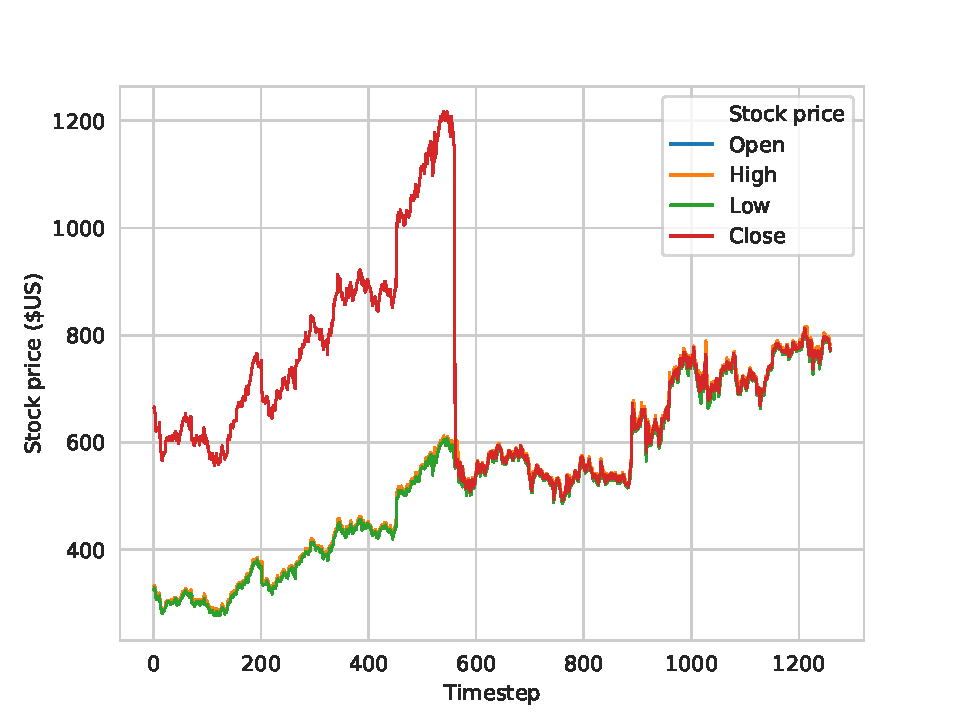
\includegraphics[width=1.0\linewidth]{stock_price.pdf}
	\end{center}
	\caption{Open, High, Low and Close prices of the Google stock (uncorrected)}
	\label{fig:price}
\end{figure}

As seen in other implementations of deep learning for stock price prediction \cite{Zhao2020,Kara2011}, the stock prices were rescaled using minimum maximum normalization to leave the stock prices from 0 to 1, using the following equation:

\begin{equation}
	x' = (b-a) \times \frac{x - min(x)}{max(x)-min(x)} + a
\end{equation}

where $b$ is the new maximum (in this case +1), $a$ in the new minimum (0), $x$ is the original feature and $x'$ is the transformed feature.

\subsubsection{Sliding window}

The prediction of time series data is usually performed using a sliding window or "look back" representation of the data. This means that the data that is used as input to predict the near future comes from the closest $n$ days (usually around 30), as the data far away from the target usually does not provide useful information for the prediction \cite{Saud2020}.

To address this issue, a sliding window approach was implemented, generating sets of explanatory variables comprising the $N$ days before the target data, and matching them with the target variable day, including the Open, Low, High and Low prices, along with the trading Volume. For practical purposes, the Date field was neglected, and only the days were there were available records were considered as part of the window.

\subsection{Gated Recurring Unit Neural Network}

To predict the stock prices, a neural network comprised of Gated recurring neural networks (GRU) was used. The GRU is comprised by two gates (reset and update). On one side, the reset gate ($r_t$) is calculated as follows \cite{Chung2014}

\begin{equation}
	r_t = \sigma (W_r x_t + U_r h_{t-1} + b_r) 
\end{equation}

where $x_t$ is the input data for time $t$, and $h_{t+1}$ is the previous hidden state $W_r$ and $U_r$ are set of weights of the gate, and $b_r$ is the bias term

While the update gate ($z_t$) is calculated as follows:

\begin{equation}
	z_t = \sigma (W_z x_t + U_z h_{t-1} + b_z) 
\end{equation}

The candidate hidden state ($\tilde{h_t}$) is calculated as 

\begin{equation}
	\tilde{h_t} = tanh(W x_t + U (r_t \odot h_{t-1} + b_z) 
\end{equation}

Finally, the output of the GRU ($h_t$) is calculated as a result of the previous output ($h_{t-1}$) and the candidate hidden state ($\tilde{h_t}$) 

The graphical summary of the above described steps can be found in Figure \ref{fig:gru} 

\begin{figure}[h]
	\begin{center}
		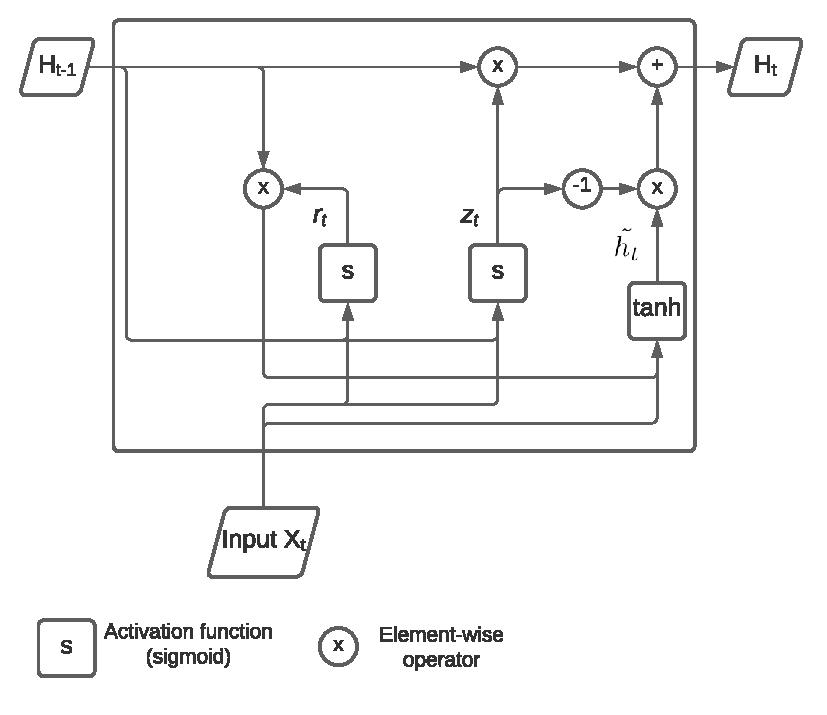
\includegraphics[width=1.0\linewidth]{GRU.pdf}
	\end{center}
	\caption{Gated Recurring Unit neural network architecture used in this study}
	\label{fig:gru}
\end{figure}

To form a neural network from the GRU, the architecture represented in Figure \ref{fig:gru_nn} was implemented. It that image it is possible to appretiate that the input data (Open, Low, High and Close prices, along with the traded volume) as a sequence is used to feed the neural network, this data is processed by multiple GRU units in the hidden layer, the oputput of these units is then directed to a fully conected that, produces five outputs (Open, Low, High, Close and Volume)

\begin{equation}
	h_t = (1-z_t) h_{t-1} + z_t \tilde{h_t}
\end{equation}

\begin{figure}[h]
	\begin{center}
		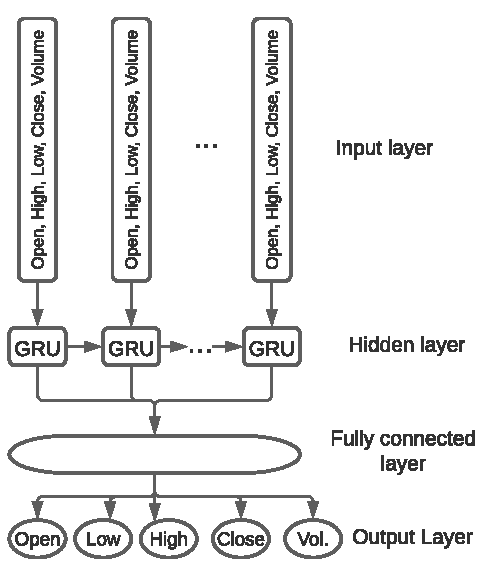
\includegraphics[width=1.0\linewidth]{GRU_nn.pdf}
	\end{center}
	\caption{Gated Recurring Unit neural network architecture used in this study}
	\label{fig:gru_nn}
\end{figure}

\subsection{Loss function and optimization criterion}

In order to train the neural network, a Mean Square Error (MSE) loss function was used:

\begin{equation}
	MSE = \frac{1}{n}\sum_{i=1}^{n} (y_i - \hat{y}_i)^2
\end{equation}

where y is the predicted stock price and $\hat{y}$ the true data

Using this loss function, backpropagation was used to update the parameters of the neural network, for the this purpose, the Adam optimizer was applied. The Adam optimizer was introduced by Kingma and Ba \cite{Kingma2015} and provides a computationally efficient method for stochastic optimization suitable for noise and sparse gradients. This optimizer is often used in the training of recurrent neural networks \cite{Zhao2020}

\subsection{Hyperparameter tuning}


In order to increase the prediction performance of the neural networks, several hyperparameters were tuned. To perform this, a validation set was created using the 20 last records of the training set (the same length as the test dataset). Using grid search (testing all the possible combination of parameters), the prediction performance of the neural network was tested on this validation dataset, and the MSE was calculated. The set of parameters with the smaller MSE was then selected for the final model.

In Table \ref{table:tuning} it is possible to see that one of the hyperparameters (window size) is belong to the preprocessing of the data in this particular problem, while the other parameters belong to the architecture of the neural network (hidden layer size, number of recurrent layers) and to the training process (number of epochs and learning rate)

\begin{table}[H]
	\begin{center}
		\begin{tabular}{|p{4.2cm}|p{3cm}|}
			\hline
			Hyperparameter & Values \\
			\hline\hline
			Window size & 20, 30, 40\\
			Hidden Layer Size & 20, 30, 40\\
			Number of recurrent layers & 1, 2, 3 \\
			Number of epochs & 500, 1000, 1500\\
			Learning rate & 0.01, 0.05, 0.001\\
			\hline
		\end{tabular}
	\end{center}
	\caption{Parameter tuning}
	\label{table:tuning}
\end{table}

\subsection{Next day and intra day prediction}

In order to test different input/output features and to increase the usability of the predictions of the neural network, three slightly different neural networks were tested. Firstly, the five features of the dataset were used as input and output (as in Figure \ref{fig:gru_nn}), and the values of these features were predicted on the next day after the last observation on the input data (nextday model). Secondly, the same architecture was tested removing the traded Volume from the input and output data, as Wang \textit{et al} \cite{Wang2003} point out that the inclusion of this variable does not help in the prediction of the Stock Price (nextday w/o Volume). 

Finally, as the trading operations are performed when the particular stock market is open (between Open and Close), a third variant, that uses the Open price to predict the Low, High and Close price on the same day was implemented. In this case, the input data is the Low, High and Close price of the $N$ days before, along with the Open price of the same day and of the $N-1 days$ before. This last variant was developed to increase the usability of the models, as it can improve the trading decision making information during the day, as having the Low, High and Close prices can help the trader decide to buy or sell the stock before the end of the day.


\section{Code and processing}

The code, along with the requirements and setup instructions for the reproduction of the above-mentioned method, can be found in the following GitHub repository: \url{https://github.com/juliancabezas/RNN-GoogleStockPrice}. All the processing was performed in a Linux OS with NVIDIA GeForce GTX 1050 with CUDA support.

\section{Results and discussion}

\subsection{Data correction}

The correction of the Close price resulted in the prices shown in Figure \ref{fig:price_corrected}, where is it possible to see that in the long term, the Google stock prices tends to increase its price, but showing several price drops in between. Lookign at the data, it is also possible to appreciate that the four prices are relatively close to each other, not showing a large intraday variations. 

\begin{figure}[h]
	\begin{center}
		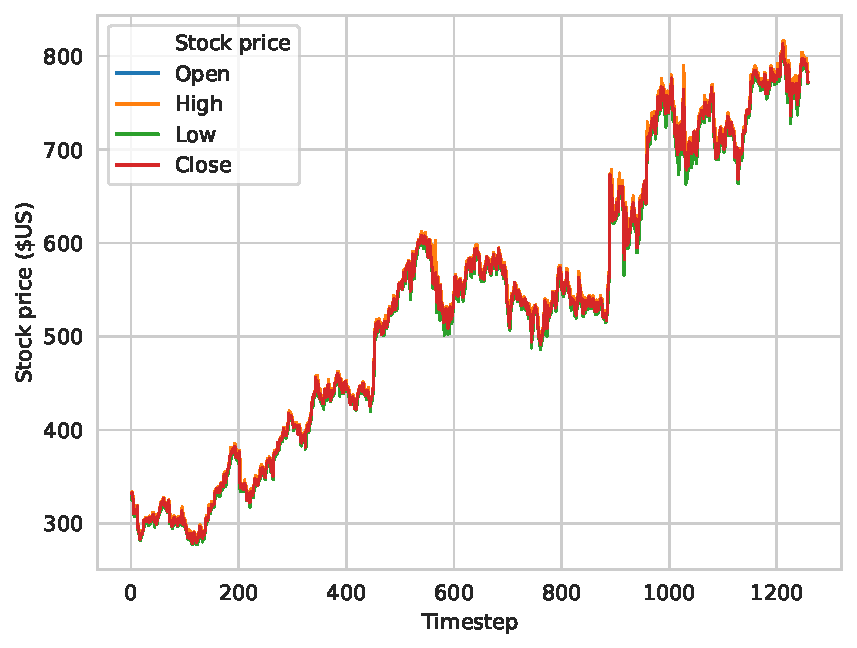
\includegraphics[width=1.0\linewidth]{stock_price_corrected.pdf}
	\end{center}
	\caption{Open, High, Low and Close prices of the Google stock (corrected)}
	\label{fig:price_corrected}
\end{figure}

On the other hand, as seen in Figure \ref{fig:volume}, the traing volume presents an erratical and noisy behaviour, with several spikes in trading.

\begin{figure}[h]
	\begin{center}
		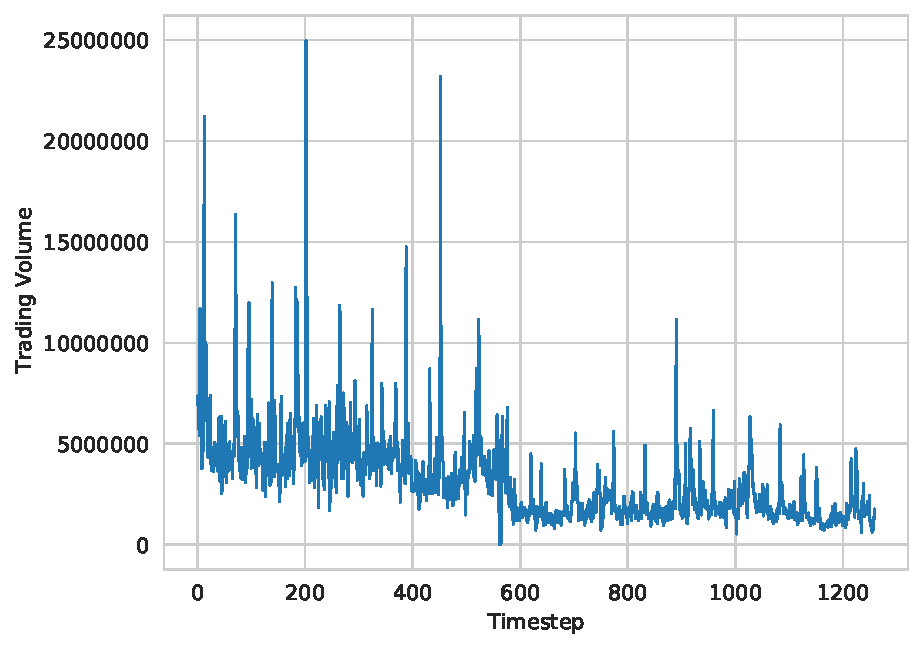
\includegraphics[width=1.0\linewidth]{volume.pdf}
	\end{center}
	\caption{Trading volume of the Google stock}
	\label{fig:volume}
\end{figure}

\subsection{Hyperparameter tuning}

The hyperparameters of the three models were (nextday, nextday w/o volume and intraday), showing the results of Table \ref{table:tuning_res}

\begin{table}[H]
	\begin{center}
		\begin{tabular}{|p{2.9cm}|p{1cm}|p{1cm}|p{1.1cm}|}
			\hline
			Hyperparameter & Nextday & Nextday w/o vol. & Intraday \\
			\hline\hline
			Window size & 40 & 30 & 40 \\
			Hidden Layer Size & 30 & 30 & 40 \\
			Number of recurrent layers & 1 & 1 & 2 \\
			Number of epochs & 1500 & 1500 & 1500 \\
			Learning rate & 0.05 & 0.05 & 0.01 \\
			\hline
		\end{tabular}
	\end{center}
	\caption{Parameter tuning results for the three tested models}
	\label{table:tuning_res}
\end{table}


\subsection{Training and testing of the final models}



\begin{figure*}[h]
	\begin{center}
		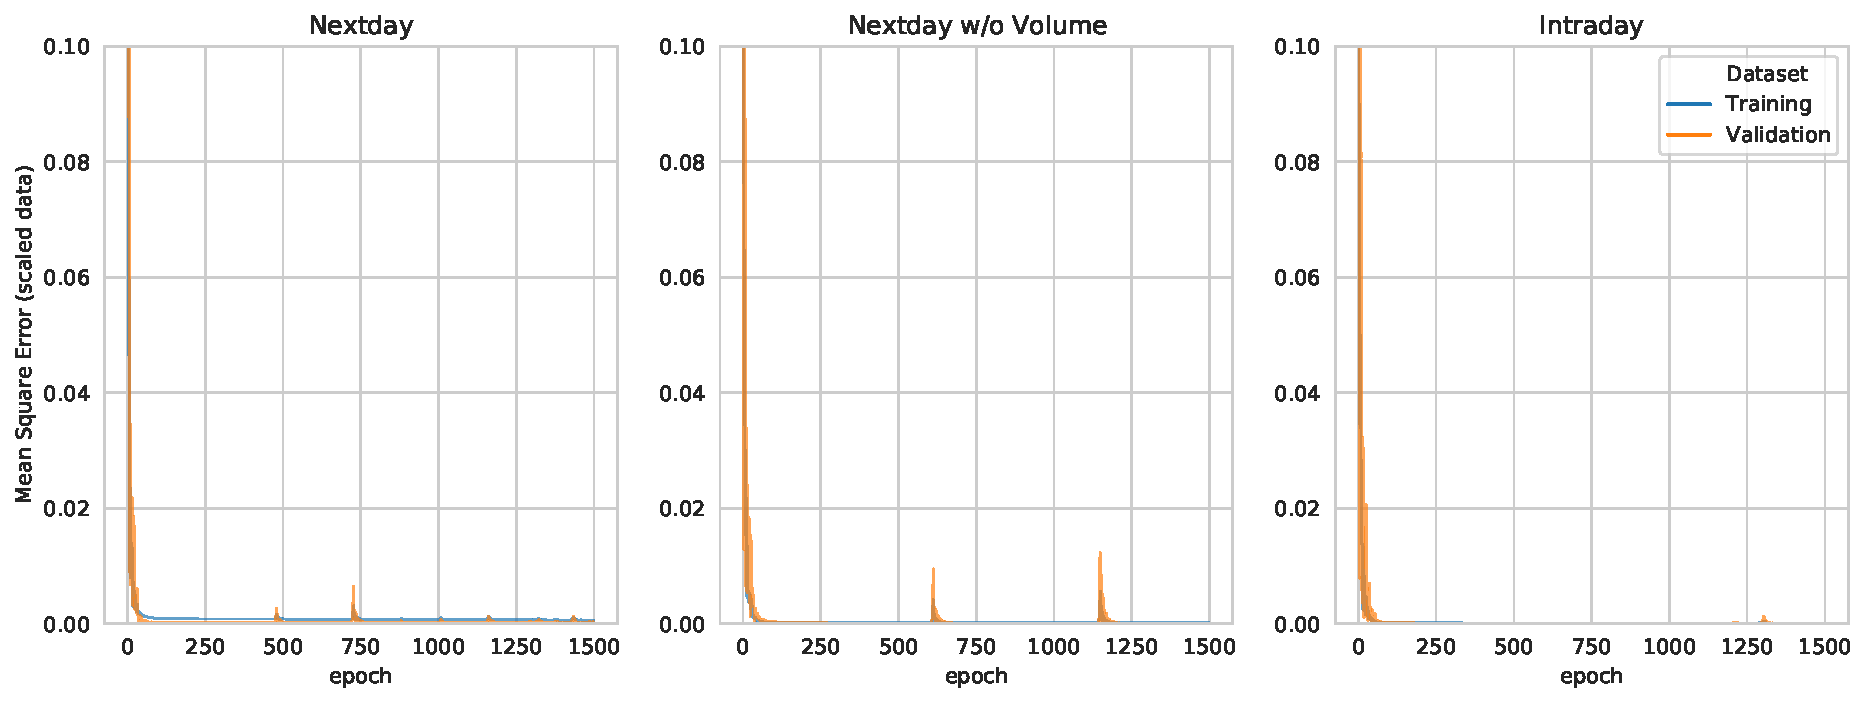
\includegraphics[width=0.9\linewidth]{train_val_loss.pdf}
		
		\caption{Training and validation loss curves for the three tested models}
		\label{fig:loss}
	\end{center}
\end{figure*}





\begin{table*}[h]
	\begin{center}
		\begin{tabular}{|p{1.8cm}|p{2cm}|p{2cm}|p{1.8cm}|p{1.8cm}|p{1.8cm}|p{1.8cm}|}
			\hline
			& \multicolumn{2}{c}{Nextday} & \multicolumn{2}{c}{Nextday w/o volume} & \multicolumn{2}{c}{Intraday} \\
			Variable & Train RMSE & Test RMSE & Train RMSE & Test RMSE & Train RMSE & Test RMSE \\
			\hline\hline
			Open price & 2.8498 & 5.9382 & 1.5054 & 5.5476 & - & - \\
			Low price & 2.6912 & 6.8495 & 2.2645 & 6.6231 & 1.8879 & 3.9610\\
			High price & 3.7242 & 6.9893 & 2.6478 & 6.8147 & 1.9452 & 4.5980 \\
			Close price & 2.9339 & 8.3147 & 2.9052 & 8.1642 & 2.4615 & 6.3192 \\
			Volume price & 954948.9845 & 1314561.2588 & - & - & - & - \\
			\hline
		\end{tabular}
	\end{center}
	\caption{Performance of the models in the test dataset}
	\label{table:error}
\end{table*}

\begin{figure}[h]
	\begin{center}
		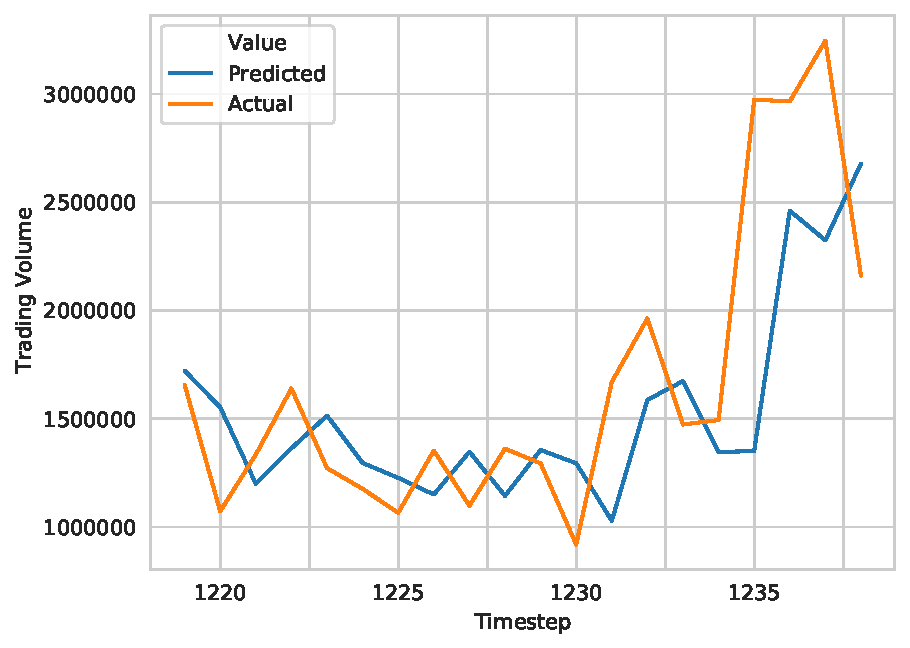
\includegraphics[width=1.0\linewidth]{prediction_volume.pdf}
	\end{center}
	\caption{Test data prediction of the trading volume of the Google stock (nextday model)}
	\label{fig:volume_pred}
\end{figure}

\begin{figure*}[h]
	\begin{center}
		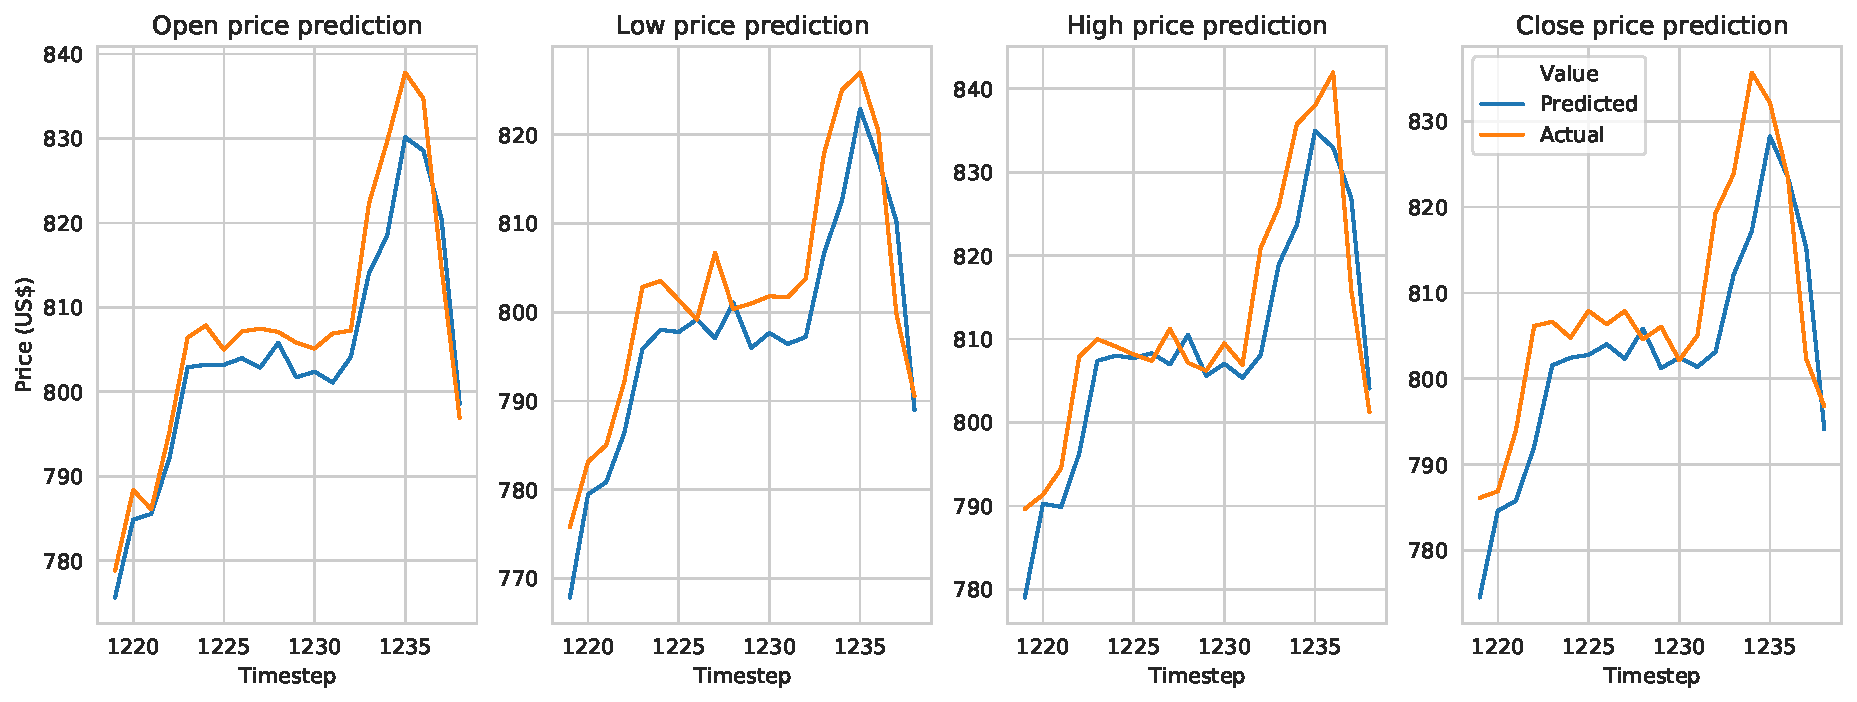
\includegraphics[width=0.9\linewidth]{prediction_nextday.pdf}
		\caption{Prediction of the nextday model for the test data}
		\label{fig:nextday_pred}
	\end{center}
\end{figure*}

\begin{figure*}[h]
	\begin{center}
		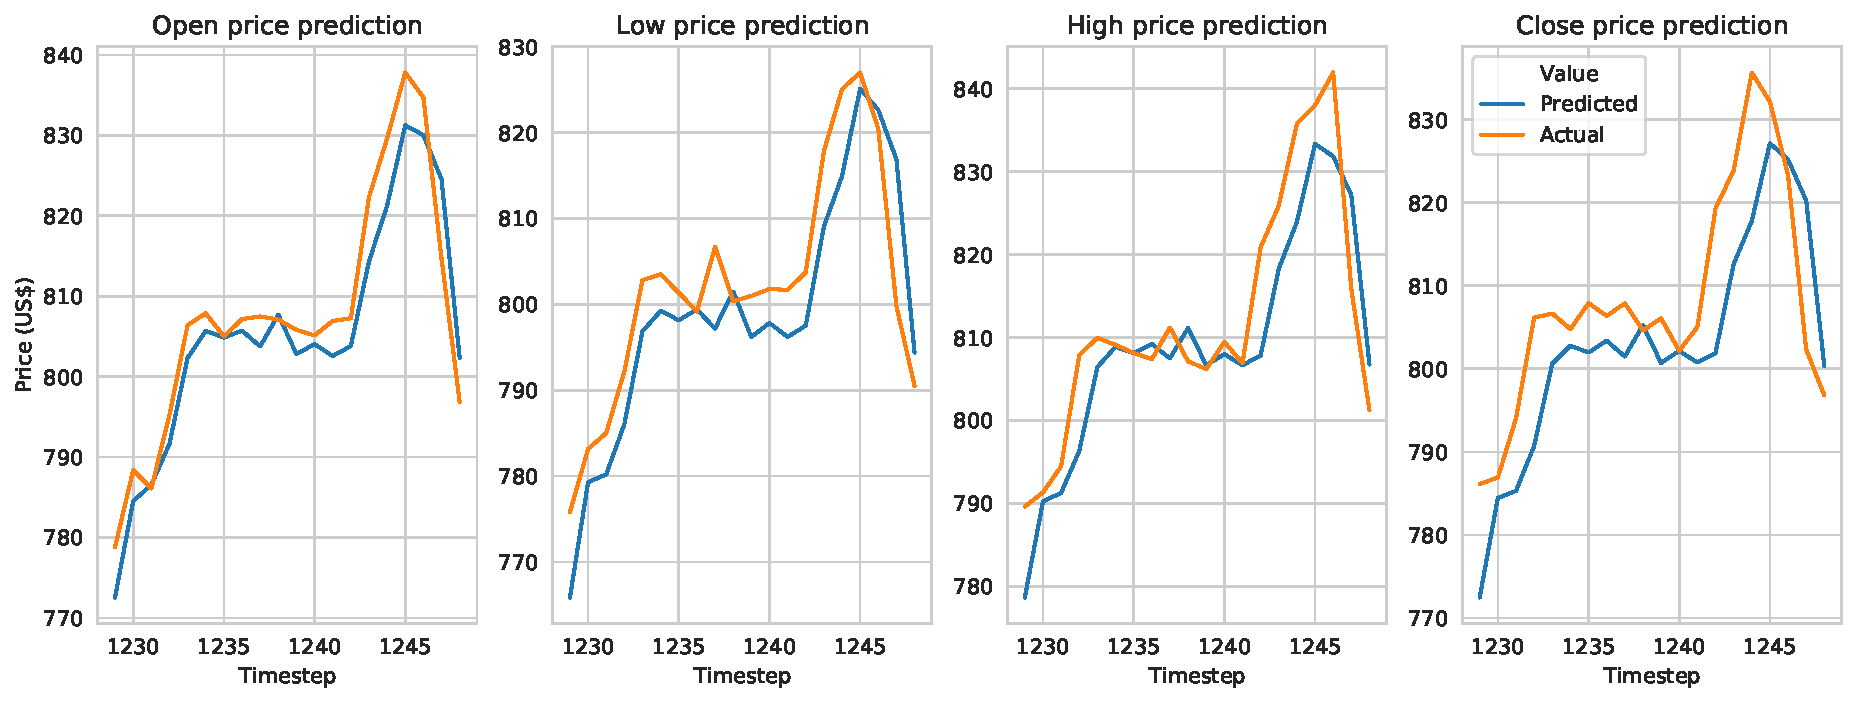
\includegraphics[width=0.9\linewidth]{prediction_nextday_novolume.pdf}
		\caption{Prediction of the nextday w/o volume for the test data}
		\label{fig:nextday_novolume_pred}
	\end{center}
\end{figure*}

\begin{figure*}[h]
	\begin{center}
		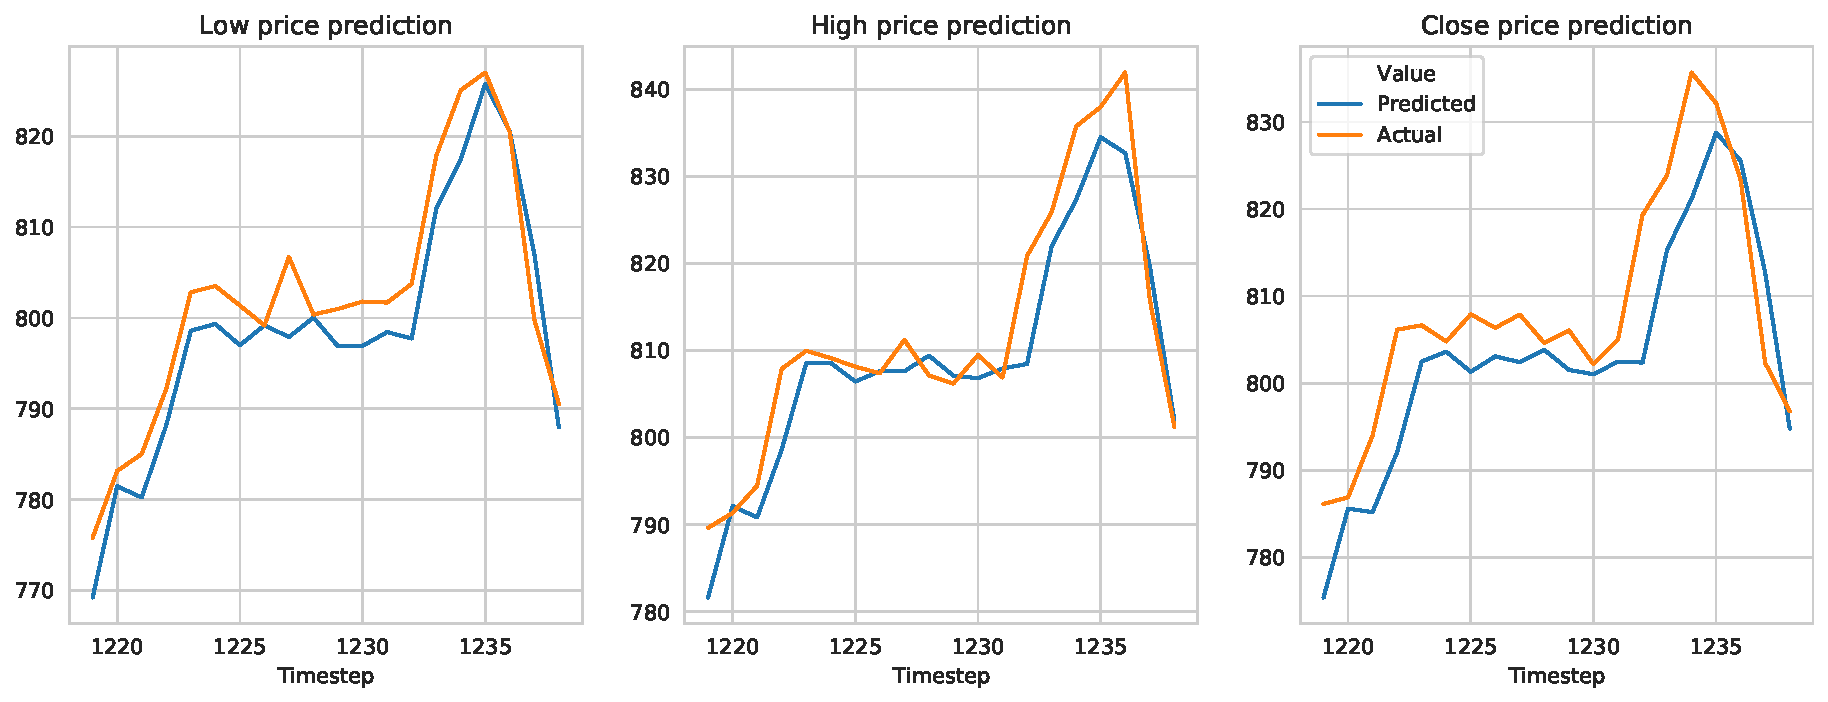
\includegraphics[width=0.9\linewidth]{prediction_intraday.pdf}
		\caption{Prediction of the nextday w/o volume for the test data}
		\label{fig:intraday_pred}
	\end{center}
\end{figure*}



\section{Conclusion}



\section{Bonus}

This research provided insight over the importance of data augmentation m

{\small
\bibliographystyle{ieee_fullname}
\bibliography{library}
}

\end{document}
